\documentclass[journal]{IEEEtai}

\usepackage[colorlinks,urlcolor=blue,linkcolor=blue,citecolor=blue]{hyperref}

\usepackage{color,array}

\usepackage{graphicx}

\usepackage{amsmath}

\usepackage{cite}

\usepackage{algpseudocode}

\usepackage{verbatim}

\usepackage{float}

\raggedbottom 

%% \jvol{XX}
%% \jnum{XX}
%% \paper{1234567}
%% \pubyear{2020}
%% \publisheddate{xxxx 00, 0000}
%% \currentdate{xxxx 00, 0000}
%% \doiinfo{TQE.2020.Doi Number}

\newtheorem{theorem}{Theorem}
\newtheorem{lemma}{Lemma}
\setcounter{page}{1}
%% \setcounter{secnumdepth}{0}


\begin{document}


\title{Tarea N° 2 {\sc Redes Neuronales} (Octubre 2023)} 


\author{Estudiante: Nicolás Araya. Profesor: Ignacio Bugeño}

\markboth{Introducción a la Inteligencia Artificial COM4402-1 - Segundo Semestre 2023}
{Introducción a la Inteligencia Artificial COM4402-1 - Segundo Semestre 2023}

\maketitle

\begin{abstract}
La inteligencia artificial (IA) se encuentra en constante evolución, y en esta transformación, las redes neuronales artificiales (RNA) desempeñan un papel fundamental. Este informe ofrece una exploración detallada de las RNA, desde sus elementos fundamentales tales como el perceptrón explicando cómo es que surge este mismo y su primer diseño Mark I \cite{Rosenblatt} que constaba de un fotoreceptor, sus capas como la capa de entrada, las capas ocultas y la capa de salida, hasta el proceso de entrenamiento explicando conceptos como las épocas, foward propagation y backward propagation. Finalizando con los resultados obtenidos en un modelo RNA aplicado al conjunto de datos \textit{Optical Recognition of Handwritten Digits Data Set} \cite{dataset}, que contiene múltiples matrices que representan dígitos escritos a mano.
Los modelos presentaron un rendimiento sólido, destacando la importancia de mantener un equilibrio en la complejidad de la arquitectura y la implementación de un eficaz método de \textit{Early Stopping}. Estos resultados subrayan la necesidad de comprender la sinergia entre los perceptrones en las RNA, lo que permite la representación de características complejas en los datos.
\end{abstract}

\begin{IEEEkeywords}
Redes Neuronales Artificiales, Perceptrón, Entrenamiento de Modelos, Funciones de Activación, Early Stopping
\end{IEEEkeywords}

\section{Introduction}

\IEEEPARstart{A}{ctualmente}, el campo de la inteligencia artificial (IA) está experimentando avances sorprendentes que están transformando radicalmente la forma en que se abordan problemas complejos en una variedad de dominios. Las redes neuronales artificiales (RNA) han emergido como una piedra angular de esta revolución, demostrando su versatilidad y eficacia en una amplia gama de aplicaciones. Desde el reconocimiento de voz hasta la visión por computadora y la toma de decisiones autónoma, las RNA han demostrado ser una herramienta de gran potencial que podría llegar a imitar y superar las capacidades humanas en tareas complejas.

Una de las aplicaciones que ayudará a ilustrar de mejor manera el potencial de las redes neuronales artificiales (RNA) corresponde a Sketch-RNN \cite{sketchrnn} herramienta que magenta permite utilizar. Esta red neuronal recurrente (RNN) es entrenada con un conjunto de datos de miles de dibujos de distintos tópicos realizados por personas en un sitio llamado QuickDraw. La red neuronal entrenada de Sketch RNN se encarga de completar un dibujo según el tipo de tópico como puede ser una cara o una actividad como yoga. Esta red neuronal con vectores de 5 dimensiones que representan posición y estado de lápiz se encarga de identificar el contexto del dibujo que el usuario está creando para finalizarlo.

Así como este ejemplo de Sketch-RNN se realizará un entrenamiento con un conjunto de datos llamado \textbf{Optical Recognition of Handwritten Digits Data Set} \cite{dataset} donde 43 personas trabajaron para la creación de los conjuntos de entrenamiento y prueba que contienen bitmaps de 32x32 que corresponden a imágenes como los QR, quiere decir  que contienen 2 colores, comunmente blanco y negro. Este entrenamiento será llevado a cabo con una red neuronal artificial simple mediante distintos modelos que contendrán distintos diseños de arquitectura que permitirán evaluar y estudiar el rendimiento de cada una.

\section{Redes Neuronales Artificiales}

\subsection{¿Qué es una Red Neuronal Artificial?}

Una Red Neuronal Artificial es un modelo computacional que consiste en un conjunto de nodos interconectados utilizados para la clasificación en diversos tipos de contextos. Los nodos que componen la RNA se llaman \textbf{perceptrones} (ver Fig. 3) y estos son creados en base al funcionamiento de las neuronas y su capacidad para el aprendizaje. Cada perceptrón toma una serie de entradas ponderadas, realiza una operación matemática en estas entradas y luego pasa la salida a través de una función de activación.

Además de los nodos (perceptrones), una Red Neuronal Artificial está compuesta de 3 capas principales (ver Fig. 1): 

\begin{enumerate}
\item	\textbf{Capa de entrada}: Esta capa es la primera capa de la red y consta de nodos que representan las características o entradas del problema. Cada nodo en esta capa está asociado con una característica de los datos de entrada. La capa de entrada recibe los datos y transmite esta información a las capas ocultas para su procesamiento.
\item	\textbf{Capa oculta}: En una red neuronal, puede haber una o varias capas ocultas, dependiendo de la arquitectura de la red. Cada capa oculta consta de un conjunto de nodos interconectados. Estos nodos realizan cálculos y transformaciones en los datos de entrada utilizando los pesos sinápticos. 
\item	\textbf{Capa de salida}: Es la última capa de la red y produce los resultados finales. Dependiendo del tipo de problema, puede haber uno o varios nodos en esta capa. Cada nodo en la capa de salida representa una posible categoría, clase o valor de salida. 
\end{enumerate}

\begin{figure}[h!]
\centering
\includegraphics[width=6cm]{img/FIGURAS/RNA.png}
\caption{Corresponde a una representación visual de la estructura completa de las RNA. Se muestran las capas de: Entrada, Oculta y de Salida.}
\label{fig: Capas RNA}
\end{figure}

\subsection{Perceptrón}

Como se mencionó anteriormente, un perceptrón corresponde a la unidad básica de una RNA, el perceptrón fue propuesto por Rosenblatt \cite{Rosenblatt} y se inspiró en la representación de un sistema neurológico llamado neurona. El perceptrón de Rosenblatt (ver Fig. 2), cuenta con una retina sensorial, compuesta por un conjunto de fotoreceptores que producían pulsos eléctricos a causa de la luz, donde las señales analógicas de la luz son procesadas y enviadas a dos áreas identificadas como las áreas de proyección que correspondería a la capa oculta del perceptrón y asociación que entregaba una respuesta binaria.

\begin{figure}[H]
\centering
\includegraphics[width=6cm]{img/FIGURAS/perceptron.png}
\caption{Representación de perceptrón de Rosenblatt \cite{Rosenblatt}. La capa de entrada correspondería a la retina, se procesaría en las áreas proyección y asociación y finalmente la capa de salida con la clasificación resultante.}
\label{fig: OriginalP}
\end{figure}

El funcionamiento de un perceptrón implica la aplicación de una función de activación al resultado de una suma ponderada para obtener la salida, denotada como $y$.
Para abordar problemas altamente no lineales y aprender representaciones más sofisticadas de los datos, se utilizan múltiples perceptrones en capas ocultas dentro de una Red Neuronal Artificial (RNA). La verdadera potencia de las RNAs radica en su capacidad para combinar y coordinar estos perceptrones en la capa oculta, permitiendo la resolución de problemas de mayor complejidad y la creación de representaciones más ricas y significativas de los datos.

\begin{figure}[H]
\centering
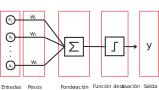
\includegraphics[width=6cm]{img/FIGURAS/fig1.png}
\caption{Diseño de un perceptrón donde \{$x_1$, $x_2$, ..., $x_n$\} corresponden a las entradas, \{$w_1$, $w_2$, ..., $w_n$\} los pesos sinápticos que se regularían para clasificar las entradas,   $\sum$ que corresponde a la suma ponderada que evalua los pesos sinápticos y finalmente $y$ que es la salida.}
\label{fig: Perceptrón}
\end{figure}

\hfill \break

\subsubsection{Suma ponderada}

La suma ponderada en una Red Neuronal Artificial se refiere a la operación en la que se calcula el valor de entrada neta a un perceptrón antes de pasar este valor a través de una función de activación. Esta suma ponderada es esencial en el procesamiento de información en una RNA y se calcula de la siguiente manera:

\begin{equation}
	f(x) = \sum{w_{i}x_{i}}  + b
\end{equation}

Donde:

\begin{itemize}
\item	$f(x)$ corresponde al valor de decisión.
\item	$x_i$ son las características de cada dato de entrada.
\item	$w_i$ son los pesos sinápticos de cada uno de los enlaces.
\item   $b$ correspondería al umbral o sesgo (bias)
\end{itemize}

Para ilustrar el concepto de suma ponderada, consideremos una tienda de muffins donde un cliente desea elegir uno para comprar. Si se encuentra algún muffin que le guste se irá de la tienda con un muffin, pero si no se irá con las manos vacias.

\begin{itemize}
    \item Muffin de Chocolate ($x_1$) = 1
    \item Muffin con Arándanos ($x_2$) = 1
    \item Muffin con Almendras ($x_3$) = 1
\end{itemize}

Para tomar una decisión más informada, asignamos un valor numérico a cada muffin que representa la preferencia personal del cliente, siendo esto el peso sináptico:

\begin{itemize}
    \item Valor del Muffin de Chocolate ($w_1$) = 3
    \item Valor del Muffin con Arándanos ($w_2$) = 4
    \item Valor del Muffin con Almendras ($w_3$) = 3
\end{itemize}
Cuando se calcula la suma ponderada de los valores de los muffins con los pesos correspondientes, se obtiene una medida de cuán atractiva es cada opción. En este caso, el muffin con arándanos tiene el mayor valor ponderado y, por lo tanto, correspondería a una opción preferida y probablemente el cliente la compraría.

Sea C un umbral que permitirá realizar la decisión del cliente:

\begin{equation}
	x_{1} * w_{1}+ x_{2} * w_{2} + x_{3} * w_{3} \geq C
\end{equation}

Escogiendo 6 como umbral, queda:

\begin{equation}
	1 * 3 + 1 * 4 + 1 * 3 \geq 6
\end{equation}

Realizando la suma:

\begin{equation}
	10 \geq 6
\end{equation}

Por lo tanto, el resultado es que el cliente se irá con un muffin de la tienda.

%%\setcounter{equation}{0}
Para llegar a la ecuación anterior (1):

\begin{equation}
	x_{1} * w_{1}+ x_{2} * w_{2} + x_{3} * w_{3} \geq C
\end{equation}

Sea $b = (-1 * C)$ la constante llamada bias:

\begin{equation}
	x_{1} * w_{1}+ x_{2} * w_{2} + x_{3} * w_{3} \geq -b
\end{equation}

Reorganizando la ecuación y expresándola en forma de suma:

\begin{equation}
	\sum{w_{i}x_{i}} + b \geq 0
\end{equation}

Entonces, el ejemplo quedaría:

\begin{equation}
	1 * 3 + 1 * 4 + 1 * 3 - 6 \geq0
\end{equation}

\begin{equation}
	4 \geq 0
\end{equation}

\subsubsection{Función de activación}

La función de activación libera del limite lineal a la Red Neuronal Artificial. Esto con el fin de realizar clasificaciones más complejas, pues el mundo real no se ve representado por modelos lineales. El resultado obtenido de la suma ponderada de cada característica multiplicada por su peso sináptico sería envíado a la función de activación, lo que permite pasar de la naturaleza lineal de la suma ponderada a una naturaleza no lineal lo que permitiría a una RNA clasificar datos como sonido, imágenes, texto, etc.

\begin{itemize}
\item Función Sigmoide:\\ \[ \sigma(z) = \frac{1}{1+e^{-z}} \] \\ Toma valores desde 0 a 1.\\ 
\item Función Tangente Hiperbólica (Tanh): \\ \[  Tanh(x) = \frac{e^{z} - e^{-z}}{e^{z} + e^{-z}} \] \\ Toma valores desde -1 a 1. \\
\item Función Rectified Linear Unit (ReLU): \\ \[  ReLU(z) = max(0, z) \] \\ Toma valores entre 0  y $+\inf$. 
\end{itemize}

\section{Entrenamiento de una RNA} 

Para el entrenamiento de cualquier modelo de aprendizaje supervisado, se debe comenzar por el pre-procesamiento de los datos y posteriormente se debe dividir el conjunto de datos en tres partes clave: el conjunto de entrenamiento, el conjunto de validación y el conjunto de prueba. Esta división es fundamental para evaluar la capacidad del modelo de generalizar a datos no vistos. \\

El entrenamiento de una RNA consta de lo siguiente:

\subsection{Épocas}

Un concepto importante a tener en cuenta son las épocas. Las épocas corresponden a un ciclo completo de entrenamiento a través de los datos de entrenamiento, lo que permite que la red ajuste sus pesos y mejore su capacidad para hacer predicciones precisas. Para que las épocas tengan sentido, constan de las siguientes etapas:
\begin{itemize}
\item	Foward Propagation: Durante la propagación hacia adelante, los datos de entrenamiento se pasan a través de la red neuronal, capa por capa, desde la entrada hasta la salida. En esta etapa, se calculan las predicciones iniciales de la red en función de los pesos actuales.
\item	Backward Propagation: En esta etapa se calculan las derivadas parciales del error con respecto a los pesos de la red. Estas derivadas se utilizan para ajustar los pesos y mejorar el rendimiento del modelo. 
\end{itemize}

\subsection{División de los Datos}

\begin{itemize}
\item	Conjunto de entrenamiento: El conjunto de entrenamiento corresponde al conjunto que se utilizará para entrenar a la Red Neuronal Artificial. 
\item	Conjunto de validación: El conjunto de validación es utilizado para evaluar el rendimiento durante el entrenamiento de la RNA.
\item	Conjunto de prueba: Este conjunto tiene los valores que se espera que la RNA prediga  y es utilizado para verificar el correcto entrenamiento de la Red Neuronal Artificial.
\end{itemize}

\subsection{Diseño de la Arquitectura}

Como se mencionó previamente, una Red Neuronal Artificial se compone de tres capas fundamentales: la capa de entrada, la capa oculta y la capa de salida. Al diseñar una RNA, es esencial especificar el número de perceptrones en cada capa y la estructura de la red. En este trabajo en particular, se optó por una configuración que consta de 64 perceptrones en la capa de entrada, lo cual permite representar las características de los datos. La capa de salida se compone de 10 perceptrones, una elección que se ajusta a la naturaleza específica de los datos en este contexto.

Es importante destacar que la capa oculta puede constar de múltiples capas y numerosos perceptrones. La clave radica en que la red sea capaz de realizar la clasificación deseada en relación con la capa de salida. El diseño de la arquitectura de la RNA es un aspecto crucial que debe adaptarse al problema y a los datos específicos que se están abordando.

\subsection{Optimizador}

El optimizador es utilizado para ajustar los pesos de la red con el objetivo de minimizar la función de costo que cuantifica la diferencia entre las predicciones de la RNA y los valores reales. Quiere decir que, por cada época, el optimizador va modificando los pesos sinápticos hasta llegar a una predicción mas cercana a los valores reales que se buscan obtener.

El optimizador utilizado en este trabajo es el llamado Adam (Adaptative Moment Estimation) \cite{Adam} que combina ventajas de los optimizadores AdaGrad (Duchi et al., 2011) y RMSProp (Tieleman \& Hinton, 2012). 

\section{Metodología}

\subsection{Herramientas}

Para la realización del trabajo se utilizó el lenguaje de Python y las librerías Scikit-Learn y PyTorch ambas librerías muy utilizadas para el entrenamiento de modelos de aprendizaje tanto supervisado como no supervisado y obtención de métricas como accuracy y matriz de confusión.

\subsection{Conjunto de datos}

El conjunto de datos a procesar corresponde a \textbf{Optical Recognition of Handwritten Digits Data Set} \cite{dataset} el cual tiene 64 características con 10 clases y 5620 muestras en total. Este conjunto de datos guarda dígitos como letras y números escritos a mano.

Se obtuvieron mediante Scikit-Learn los datos de validación. Estos fueron normalizados mediante el método StandarScaler() y procesados con numpy para la obtención de los labels a utilizar para el entrenamiento de la Red Neuronal Artificial.

\subsection{Diseño de la Arquitectura}

Código que muestra cómo se diseño la arquitectura base con torch:
\begin{flalign*}
\hline
& \text{model} = \text{nn.Sequential (} \\
&\quad \text{nn.Linear(}64, 10 \text{),} \\
&\quad \text{nn.ReLU(),} \\
&\quad \text{nn.Linear(}10,10\text{),} \\
&\quad \text{)} \\
\hline
\end{flalign*}
\begin{verbatim}
	
\end{verbatim}

Código de creación de modelos RNA:

\begin{figure}[h!]
\centering
\includegraphics[width=8cm]{img/CODES/models.png}
\caption{Código creado para la creación de modelos RNA. Guarda en una lista las funciones y las ordena según la lógica de nn.Sequential para formar el modelo.}
\label{fig: RNAMODELSCODE}
\end{figure}

\subsection{Entrenamiento}

\begin{figure}[h!]
\centering
\includegraphics[width=8cm]{img/CODES/eval.png}
\caption{En el código se itera por cada época que es especificada por el Usuario. Se inicializa el entrenamiento con model.train() y dentro de una época se iteran los valores entregados por dataloader\_train correspondiente al conjunto de datos de entrenamiento procesado para la RNA. Dentro de la iteración del dataloader se procesan los labels, se realizan foward propagation, la optimización y backward propagation.}
\label{fig: RNATRAINMODEL}
\end{figure}

Como se mencionó anteriormente, al entrenar una RNA se deben definir una cantidad adecuada de épocas (ver Fig. 5), ya que, por cada época la red neuronal se retroalimenta mediante Foward Propagation, Backward Propagation y el Optimizer. El número de épocas es un hiperparámetro crítico que debe ajustarse cuidadosamente. Demasiadas épocas pueden llevar a un sobreajuste (overfitting), donde la RNA se adapta demasiado a los datos de entrenamiento y no generaliza bien a nuevos datos. Es por ello que se debe encontrar una manera de detener el entrenamiento en el momento que se tope con la mejor predicción posible.

\subsection{Early Stopping}

En cada época, se registra el valor de las variables \textbf{validation loss} y \textbf{training loss} (ver Fig. 6),  que representan la pérdida de validación y la pérdida de entrenamiento, respectivamente. Estas métricas cuantifican cuán alejadas están las predicciones de la red neuronal de los valores reales en los conjuntos de validación y entrenamiento, proporcionando una evaluación importante del desempeño del modelo. 

La técnica de "Early Stopping" requiere una condición que permita detener el entrenamiento de manera anticipada con el propósito de conservar la mejor predicción obtenida hasta ese momento.

\begin{figure}[h!]
\centering
\includegraphics[width=8cm]{img/FIGURAS/earlystoping.png}
\caption{\textbf{Validation loss} y \textbf{Training loss} se encuentran en el punto óptimo cuando validation loss es lo más cercano a 0 posible permitido por el modelo RNA. \textbf{Training loss} va disminuyendo a medida que se es entrenada la RNA lo que permite detectar sobreajustes y en caso de haberlos, se debe reiniciar el modelo RNA, ajustar hiperparámetros si es necesario y entrenarlo nuevamente.}
\label{fig: EARLYSTOP}
\end{figure}

El método de Early Stopping formulado para este trabajo es el siguiente:
\setcounter{equation}{0}
\begin{flalign*}
\hline
&patience  \leftarrow 20 \\
&wait \leftarrow 0  \\
&\text{\textbf{if}} \quad [current\_loss\_val - last\_loss\_val] < 0 \quad \text{\textbf{then}} \\
&\quad last\_loss\_val \leftarrow current\_loss\_val \\
&\quad wait \leftarrow 0 \\
&\text{\textbf{else}} \\
&\quad wait \leftarrow wait  + 1 \\
&\quad \text{\textbf{if}} \quad wait \geq patience \quad \text{\textbf{then}} \\
&\quad \quad break \\
&\quad \text{\textbf{endif}} \\
&\text{\textbf{endif}} \\
\hline
\end{flalign*}

\hfill \break

Esta técnica se basa en el seguimiento de la diferencia entre las pérdidas de validación en épocas consecutivas. La idea principal es que, durante un entrenamiento exitoso, el loss validation disminuirá en cada época, lo que resultará en una diferencia positiva entre la pérdida actual y la pérdida anterior. Sin embargo, si la RNA comienza a sobreajustar, es probable que loss validación aumente, lo que dará como resultado una diferencia negativa entre la pérdida actual y la pérdida anterior. 

\subsection{Guardar los modelos}

Se realizó la siguiente estructura para guardar cada modelo junto a sus resultados y características correspondientes:

\begin{align*}
\hline
&\text{Results} \leftarrow (\\
&\quad name \\
&\quad model \\
&\quad optimizer \\
&\quad loss\_train \\
&\quad epochs \\
&\quad time  \\
&\quad accuracies \\
&\quad predictions \\
&\quad confusion\_matrix )\\
\hline
\end{align*}

\subsection{Modelos Utilizados}

Los modelos creados para su posterior entrenamiento son los siguientes:

\begin{itemize}
\item[a)]	10 neuronas en la capa oculta, usando función de activación ReLU y 1000 épocas como máximo.
\item[b)]	40 neuronas en la capa oculta y función de activación ReLU, y 1000 épocas como máximo.
\item[c)]	10 neuronas en la capa oculta y función de activación Tanh, y 1000 épocas como máximo.
\item[d)] 40 neuronas en la capa oculta y función de activación Tanh, y 1000 épocas como máximo.
\item[e)] 2 capas ocultas con 10 y 10 neuronas cada una y función de activación ReLU, y 1000 épocas como máximo.
\item[f)] 2 capas ocultas con 40 y 40 neuronas cada una y función de activación ReLU, y 1000 épocas como máximo.
\end{itemize}

\section{Resultados}

Para poder representar de una forma más corta e intuitiva los modelos, el nombre de cada modelo fue formulado de la siguiente manera:

\begin{itemize}
\item	model1\_50HReLU 
\end{itemize}

Nos indica que es un modelo que tiene solamente 50 perceptrones en una capa oculta y utiliza la función de activación ReLU. 

\begin{figure}[H]
\centering
\includegraphics[width=8cm]{img/model10HReLU/lossvsval.png}
\caption{Loss vs Validation. Se muestra el término de entrenamiento del RNA: model1\_10HReLU}
\label{fig: model110HReLULOSSVSVAL}
\end{figure}

\begin{figure}[H]
\centering
\includegraphics[width=8cm]{img/model10HReLU/train.png}
\caption{El conjunto de entrenamiento vs las predicciones de este modelo entregó un accuracy score normalizado de  0.9895. La matriz de confusión muestra que los resultados son bastante aceptables: model1\_10HReLU}
\label{fig: model110HReLUTRAIN}
\end{figure}

\begin{figure}[H]
\centering
\includegraphics[width=8cm]{img/model10HReLU/val.png}
\caption{El conjunto de validación vs las predicciones de este modelo entregó un accuracy score normalizado de  0.9625. La matriz de confusión muestra que los resultados son bastante aceptables: model1\_10HReLU}
\label{fig: model110HReLUVAL}
\end{figure}

\begin{figure}[H]
\centering
\includegraphics[width=8cm]{img/model40HReLU/lossvsval.png}
\caption{Loss vs Validation. Se muestra el término de entrenamiento del RNA: model1\_40HReLU}
\label{fig: model140HReLULOSSVSVAL}
\end{figure}

\begin{figure}[H]
\centering
\includegraphics[width=8cm]{img/model40HReLU/train.png}
\caption{El conjunto de entrenamiento vs las predicciones de este modelo entregó un accuracy score normalizado de  1. La matriz de confusión muestra que los resultados son perfectos: model1\_40HReLU}
\label{fig: model140HReLUTRAIN}
\end{figure}

\begin{figure}[H]
\centering
\includegraphics[width=8cm]{img/betterAccuracyModel/val.png}
\caption{El conjunto de validación vs las predicciones de este modelo entregó un accuracy score normalizado de  0.9755. La matriz de confusión muestra que los resultados son bastante aceptables: model1\_40HReLU}
\label{fig: model140HReLUVAL}
\end{figure}

\begin{figure}[H]
\centering
\includegraphics[width=8cm]{img/model10HTanh/lossvsval.png}
\caption{Loss vs Validation. Se muestra el término de entrenamiento del RNA: model1\_10HTanh}
\label{fig: model110HTanhLOSSVSVAL}
\end{figure}

\begin{figure}[H]
\centering
\includegraphics[width=8cm]{img/model10HTanh/train.png}
\caption{El conjunto de entrenamiento vs las predicciones de este modelo entregó un accuracy score normalizado de  0.9924. La matriz de confusión muestra que los resultados son perfectos: model1\_10HTanh}
\label{fig: model110HTanhTRAIN}
\end{figure}

\begin{figure}[H]
\centering
\includegraphics[width=8cm]{img/model10HTanh/val.png}
\caption{El conjunto de validación vs las predicciones de este modelo entregó un accuracy score normalizado de  0.9648. La matriz de confusión muestra que los resultados son bastante aceptables: model1\_10HTanh}
\label{fig: model110HTanhVAL}
\end{figure}

\begin{figure}[H]
\centering
\includegraphics[width=8cm]{img/model40HTanh/lossvsval.png}
\caption{Loss vs Validation. Se muestra el término de entrenamiento del RNA: model1\_40HTanh}
\label{fig: model140HTanhLOSSVSVAL}
\end{figure}

\begin{figure}[H]
\centering
\includegraphics[width=8cm]{img/model40HTanh/train.png}
\caption{El conjunto de entrenamiento vs las predicciones de este modelo entregó un accuracy score normalizado de  0.9997. La matriz de confusión muestra que los resultados son perfectos: model1\_40HTanh}
\label{fig: model140HTanhTRAIN}
\end{figure}

\begin{figure}[H]
\centering
\includegraphics[width=8cm]{img/model40HTanh/val.png}
\caption{El conjunto de validación vs las predicciones de este modelo entregó un accuracy score normalizado de  0.9762. La matriz de confusión muestra que los resultados son bastante aceptables: model1\_40HTanh}
\label{fig: model140HTanhVAL}
\end{figure}

\begin{figure}[H]
\centering
\includegraphics[width=8cm]{img/model210HReLU/lossvsval.png}
\caption{Loss vs Validation. Se muestra el término de entrenamiento del RNA: model2\_10HReLU}
\label{fig: model210HReLULULOSSVSVAL}
\end{figure}

\begin{figure}[H]
\centering
\includegraphics[width=8cm]{img/model210HReLU/train.png}
\caption{El conjunto de entrenamiento vs las predicciones de este modelo entregó un accuracy score normalizado de  0.9928. La matriz de confusión muestra que los resultados son perfectos: model2\_10HReLU}
\label{fig: model210HReLUTRAIN}
\end{figure}

\begin{figure}[H]
\centering
\includegraphics[width=8cm]{img/model210HReLU/val.png}
\caption{El conjunto de validación vs las predicciones de este modelo entregó un accuracy score normalizado de  0.9548. La matriz de confusión muestra que los resultados son bastante aceptables: model2\_10HReLU}
\label{fig: model210HReLUVAL}
\end{figure}

\begin{figure}[H]
\centering
\includegraphics[width=8cm]{img/model240HReLU/lossvsval.png}
\caption{Loss vs Validation. Se muestra el término de entrenamiento del RNA: model2\_40HReLU}
\label{fig: model240HReLULOSSVSVAL}
\end{figure}

\begin{figure}[H]
\centering
\includegraphics[width=8cm]{img/model240HReLU/train.png}
\caption{El conjunto de entrenamiento vs las predicciones de este modelo entregó un accuracy score normalizado de  0.9997. La matriz de confusión muestra que los resultados son perfectos: model2\_40HReLU}
\label{fig: model240HReLUTRAIN}
\end{figure}

\begin{figure}[H]
\centering
\includegraphics[width=8cm]{img/model240HReLU/val.png}
\caption{El conjunto de validación vs las predicciones de este modelo entregó un accuracy score normalizado de  0.9739. La matriz de confusión muestra que los resultados son bastante aceptables: model2\_40HReLU}
\label{fig: model240HReLUVAL}
\end{figure}

\section{Análisis}

\subsection{Modelo con mayor accuracy en validación}

El modelo que mayor accuracy en validación presentó fue model1\_40HReLU (ver Fig. 18) , para comprobar que en realidad es bueno. Usando el conjunto de prueba para obtener la matriz de confusión normalizada y el accuracy normalizado (ver Fig. 25) podemos entender qué tan bien entrenado quedó el modelo RNA, ya que el conjunto de prueba nos permite ver su rendimiento en datos que no han sido utilizados durante el entrenamiento. 
Nos permite comprobar que mientras mayor sea el accuracy de validación es muy probable que el accuracy en el conjunto de datos de prueba también sea adecuado e incluso mejor que el accuracy de validación.

\begin{figure}[H]
\centering
\includegraphics[width=8cm]{img/betterAccuracyModel/test.png}
\caption{El conjunto de prueba vs las predicciones de este modelo entregó un accuracy score normalizado de  0.9811. La matriz de confusión muestra que los resultados son bastante aceptables: model1\_40HReLU}
\label{fig:  model140HTanhTEST}
\end{figure}

\subsection{Perceptrones}

Aunque en el trabajo todos los modelos hayan tenido un buen rendimiento mostrado en cada una de las matrices de confusión, se tiene que el modelo RNA model1\_40HReLU, teniendo 64 neuronas de entrada, solo 40 neuronas en la capa oculta y 10 neuronas de salida tuvo un rendimiento un poco superior al resto. 

Para entender mejor a qué puede deberse, se analizarán los dos extremos para entender los efectos de variar la cantidad de neuronas en la capa oculta y cómo afecta al desempeño de la red.

\subsubsection{Un solo perceptrón}

Un ejemplo adecuado correspondería al caso en que la RNA está conformada por un simple perceptrón de múltiples entradas y una sola salida, pues los resultados de un solo perceptrón son binarios y tendería a perder características. (ver Fig. 27)

El primer argumento que respalda que un modelo de este tipo no es el adecuado para representar bien la complejidad del conjunto de datos corresponde a la combinación lineal de las entradas con la formula de la suma ponderada explicada anteriormente en la ecuación (1).

\setcounter{equation}{0}
\begin{equation}
	f(x) = \sum{w_{i}x_{i}}  + b
\end{equation}

Luego de que la suma ponderada pasa por la función de activación, el resultado final se vuelve no lineal debido a la función de activación. Sin embargo, es importante tener en cuenta que este proceso no lineal se basa en un cálculo que es bastante sencillo. Por esta razón, para manejar con éxito sistemas que involucran muchas características y hacer una clasificación precisa, es necesario usar varios perceptrones que trabajen juntos. Cada perceptrón contribuye con su propio tipo de procesamiento no lineal y, al combinar los resultados de varios perceptrones, se obtiene una representación más completa y detallada de los datos, lo que hace que la red sea mucho mejor para hacer tareas de clasificación. (ver Fig. 26).

\begin{figure}[H]
\centering
\includegraphics[width=8cm]{img/exp/1p.png}
\caption{Corresponde a la matriz de confusión al aplicar un solo perceptrón en la capa oculta.}
\label{fig: 1p}
\end{figure}

\subsubsection{Gran cantidad de perceptrones}

Con una gran cantidad de perceptrones, las características no se pierden durante el entrenamiento, aunque mientras más perceptrones en las capas ocultas más recursos computacionales serán requeridos y por ende más tiempo. Mediante el entrenamiento de varios modelos con diferentes cantidades de neuronas (ver Fig. 27 y 28) se puede comprobar también la irrelevancia de tener una gran cantidad de perceptrones en las capas ocultas.

\begin{figure}[H]
\centering
\includegraphics[width=8cm]{img/exp/hipperExpBig.png}
\caption{Se entrenan 100 modelos mediante una iteración que incrementa la cantidad de neuronas en la capa oculta. Se obtiene como resultado que una gran cantidad de perceptrones causa que la duración sea bastante alta debido a la cantidad de recursos.}
\label{fig: expBig}
\end{figure}


\begin{figure}[H]
\centering
\includegraphics[width=8cm]{img/exp/onlyAcc.png}
\caption{Corresponde al accuracy vs perceptrones. Se observa que se mantiene sobre el 90\% y podría tender a disminuir a medida que aumentan los perceptrones.}
\label{fig: expBig}
\end{figure}

\subsection{Capas Ocultas}

Además de evaluar según la cantidad de perceptrones en una sola capa oculta, es importante entender el cambio que existe al variar la cantidad de capas ocultas por lo que se procedió a evaluar una cantidad constante de perceptrones, especificamente 40 perceptrones con la función de activación ReLU en base al modelo obtenido con mejor desempeño, pero con un aumento gradual de capas ocultas. El resultado fue que a mayor cantidad de capas ocultas, menor sería el accuracy (ver Fig. 29).

\begin{figure}[h!]
\centering
\includegraphics[width=8cm]{img/exp/layersExp.png}
\caption{En este gráfico se muestra la disminución abrupta de accuracy a medida que aumentan las capas ocultas hasta llegar a una cantidad de 100 capas ocultas.}
\label{fig: layersExp}
\end{figure}

\subsection{Funciones de activación implementadas}

Como se pudo ver en los resultados, fueron aplicadas ReLU y Tanh en los modelos RNA. Ambas funciones de aplicación rindieron bastante bien, pero ReLU fue superior (ver Fig. 30) esto debido a la naturaleza de los datos dado que ReLU se apaga en valores negativos y es efectivo para eliminar características no deseadas o ruido en los datos, lo que puede ser beneficioso en este tipo de aplicaciones a diferencia de Tanh que puede generar salidas en un rango de valores desde -1 hasta 1 por lo que permitirá algo de ruido al momento de clasificar esas matrices.

\begin{figure}[h!]
\centering
\includegraphics[width=8cm]{img/exp/ReLUvsTanh.png}
\caption{El accuracy resultante de ReLU es mejor que el de Tanh en el entrenamiento de este conjunto de datos.}
\label{fig: ReLUvsTanh}
\end{figure}

\subsection{Evaluación de modelos}

\subsubsection{ReLU}

\hfill \break

\begin{tabular}{| c | c | c |}
\hline
Modelo & Dt & Validation Accuracy \\
\hline
model1\_10HReLU & 16 seg & 96.25 \% \\
model1\_40HReLU & 7 seg & 97.62 \% \\
model2\_10HReLU & 5.7 seg & 95.48 \% \\
model2\_40HReLU & 3 seg & 97.39 \% \\
\hline
\end{tabular} \\

\subsubsection{Tanh}

\hfill \break

\begin{tabular}{| c | c | c |}
\hline
Modelo & Dt & Validation Accuracy \\
\hline
model1\_10HTanh& 7.6 seg & 96.48 \% \\
model1\_40HTanh & 6.5 seg & 97.62 \% \\
\hline
\end{tabular} \\

Los modelos con función ReLU lograron un rendimiento superior en términos de precisión de validación en comparación con los modelos Tanh. En particular, el modelo model1\_40HReLU obtuvo la mayor precisión del 97.62\%, seguido de cerca por model2\_40HReLU con 97.39\%. En contraste, el modelo model1\_40HTanh logró una precisión similar, pero el tiempo de entrenamiento fue más corto que el modelo ReLU equivalente.

\subsubsection{Matrices de Confusión}

Las matrices de confusión revelan un alto valor en los verdaderos positivos (TP) en todos los modelos, lo que demuestra una fuerte capacidad para clasificar correctamente los dígitos escritos a mano. El modelo model1\_40HReLU con función ReLU alcanzó el 97.62\% de precisión y un alto número de verdaderos positivos (ver Fig. 12). Similarmente, el modelo model2\_40HReLU también logró un elevado número de TP con una precisión del 97.39\% (ver Fig. 24). En el caso de Tanh, el modelo model1\_40HTanh obtuvo una precisión comparable, pero con un tiempo de entrenamiento más corto (ver Fig. 18).

Respecto a los modelos con dos capas ocultas, estos también tuvieron un buen rendimiento y tardaron incluso menos, pero la precisión sigue siendo menor que aquellos modelos con una sola capa oculta.

\section{Conclusiones generales}

En resumen, los modelos presentados exhibieron un rendimiento sólido, con una precisión general superior al 90\% y con un tiempo de término1 bastante aceptable. Cabe considerar ampliamente que corresponde tener más de una capa oculta, pues permite que el modelo acabe antes su entrenamiento y no disminuye mucho su rendimiento. Los resultados destacaron la importancia de factores clave en el diseño de la arquitectura de las redes neuronales artificiales (RNA) que influye significativamente en el rendimiento de los modelos. El equilibrio en la complejidad de la arquitectura es fundamental, evitando tanto una cantidad excesiva de capas ocultas y perceptrones, que puede aumentar significativamente el consumo de recursos computacionales, como una arquitectura demasiado simple, que puede limitar la capacidad de la RNA para aprender patrones complejos en los datos.
Además, se destacó la utilidad de un método de \textbf{Early Stopping} para determinar el momento óptimo de finalización en el entrenamiento de la RNA, evitando el sobreajuste de los modelos.
Por último, se enfatizó la sinergia presente entre los perceptrones en la RNA, ya que cada resultado de un perceptrón se procesa con los pesos sinápticos hacia los perceptrones siguientes, lo que permite un aprendizaje colaborativo y la representación de características complejas en los datos.

\section*{Bibliografía}
\def\refname{}
\begin{thebibliography}{34}
	\bibitem{RNA} Izaurieta, F., \& Saavedra, C. (2000). Redes neuronales artificiales. Departamento de Física, Universidad de Concepción Chile.
	\bibitem{Rosenblatt} Rosenblatt, F. (1958). The perceptron: A probabilistic model for information storage and organization in the brain. Psychological Review, 65(6), 386–408. doi:10.1037/h0042519 
	\bibitem{Perceptron} Block, H. D. (1962). The Perceptron: A Model for Brain Functioning. I. Reviews of Modern Physics, 34(1), 123–135. doi:10.1103/revmodphys.34.123
	\bibitem{Adam} Kingma, D. P., \& Ba, J. (2014). Adam: A method for stochastic optimization. arXiv preprint arXiv:1412.6980.
	\bibitem{sketchrnn} David Ha and Douglas Eck. (2017). A Neural Representation of Sketch Drawings. arXiv preprint arXiv:1704.03477.
	\bibitem{dataset} Alpaydin,E. and Kaynak,C.. (1998). Optical Recognition of Handwritten Digits. UCI Machine Learning Repository. https://doi.org/10.24432/C50P49.
\end{thebibliography}

\end{document}
